\documentclass{article}
\usepackage{amsmath,amsfonts,tikz}
\title{MATH 322 Assignment 1}
\author{Oliver Tonnesen\\V00885732}
\date{January 24, 2019}
\begin{document}
\maketitle
\renewcommand{\thesubsection}{\thesection.\alph{subsection}}
\section{} % Section 1
\subsection{} % Section 1.a
We present such a list:\\
$\{1,2,3\},\{1,2,4\},\{1,2,5\},\{1,2,6\},\{1,3,6\},\{2,3,6\},\{2,3,5\},\{2,3,4\},\\
\{1,3,4\},\{1,3,5\},\{1,4,5\},\{1,4,6\},\{1,5,6\},\{2,5,6\},\{2,4,6\},\{2,4,5\},\\
\{3,4,5\},\{3,4,6\},\{3,5,6\},\{4,5,6\}$
\subsection{} % Section 1.b
We present a graph representing the adjacencies:
\newline
\newline
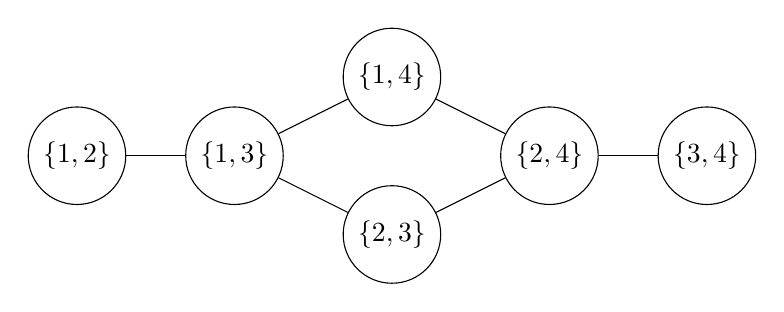
\begin{tikzpicture}
	\node[circle,draw] (12) at (0,0)	{$\{1,2\}$};
	\node[circle,draw] (13) at (2,0)	{$\{1,3\}$};
	\node[circle,draw] (14) at (4,1)	{$\{1,4\}$};
	\node[circle,draw] (23) at (4,-1)	{$\{2,3\}$};
	\node[circle,draw] (24) at (6,0)	{$\{2,4\}$};
	\node[circle,draw] (34) at (8,0)	{$\{3,4\}$};

	\path (12) edge node {} (13);
	\path (13) edge node {} (14);
	\path (13) edge node {} (23);
	\path (14) edge node {} (24);
	\path (23) edge node {} (24);
	\path (24) edge node {} (34);
\end{tikzpicture}
\newline
\newline
This graph clearly has no Hamiltonian path, and so no such list exists.
\subsection{} % Section 1.c
Let $A_1,A_2,...,A_t$ be $k$-subsets of $[n]$. We'll use $\sim$ to represent
adjacency for the remainder of the proof.
\newline
\newline
Suppose $A_1\sim A_2$ and $A_2\sim A_3$ and $A_1\neq A_3$. Then either $A_3$
differs from $A_2$ in the same spot as $A_1$, but going in the opposite
direction (for example, $A_1=\{3,5\}$, $A_2=\{3,6\}$, $A_3=\{3,7\}$), or $A_3$
differs from $A_2$ in a different spot than $A_1$ (for example, $A_1=\{3,5\}$,
$A_2=\{3,6\}$, $A_3=\{2,6\}$). In any case, $A_1\not\sim A_3$ if $A_3\sim A_2$
and $A_2\sim A_1$. So no neighbor of a neighbor of $A_1$ can be a neighbor of
$A_1$. This is true of any $A\subseteq[n]$, $|A|=k$. So we consider the graph
representing this system. It is clearly 2-colourable given its properties, and
so there exists a bipartition of the $k$-subsets of $[n]$.
\section{} % Section 2
Let us chooose a representative for each of the $n$ groups, and count how many
options we have at the time:
\newline
\newline
$A_1$: We choose either of the two elements, and call it $x_1$.
\newline
$A_2$: Suppose that $A_1\subset A_2$. Then we cannot choose $x_1$, so we
choose either of the remaining two elements, and call it $x_2$. Notice that if
$A_1\not\subset A_2$, then we have more than two choices.
\newline
$A_2$: Suppose that $A_2\subset A_3$. Then we cannot choose $x_1$ or $x_2$, so we
choose either of the remaining two elements, and call it $x_3$. Notice that if
$A_2\not\subset A_3$, then we have more than two choices.
\newline
$\vdots$
\newline
$A_n$: Suppose that $A_{n-1}\subset A_n$. Then we cannot choose any of
$x_1,x_2,\ldots,x_{n-1}$, so we choose either of the remaining two elements,
and call it $x_n$.
\newline
\newline
Notice that at each of the $n$ steps, we had at least two options for which
element to choose. Then, by the law of product, there were at least $2^n$ ways
we could have chosen our SDR.
\section{} % Section 3
\subsection{} % Section 3.a
Claim: There is an SDR which includes $a_1,a_2,\ldots,a_t$ (but not necessarily
as representatives for $A_1,A_2,\ldots,A_t$).
\newline
Proof: [Induction on $t$]
\newline
Base: $t=1$: Given that $A_1$ has an SDR, this is trivially true.
\newline
Induction Hypothesis: Suppose there exists some $k$ such that we can construct
an SDR for $A_1,A_2,\ldots,A_n$ containing $a_1,a_2,\ldots,a_l$ for all $l\le k$.
\newline
Induction Step: We attempt to construct an SDR for $A_1,A_2,\ldots,A_n$ containing
$a_1,a_2,\ldots,a_{k+1}$ given some $a_{k+1}\in A_{k+1}$:
\newline
By the induction hypothesis, we know that there exists an SDR for
$A_1,A_2,\ldots,A_n$ containing $a_1,a_2,\ldots,a_k$. Given this, we can construct
an SDR for $A_1,A_2,\ldots,A_{k+1}$ containing $a_{k+1}$ as follows:
\newline
Case 1: $a_{k+1}$ is already the representative for $A_{k+1}$: Done.
Case 2: $a_{k+1}$ is not the representative for $A_{k+1}$: Replace the current
representative for $A_{k+1}$ with $a_{k+1}$. If the resulting tuple is an SDR,
then we're done. If not, then $a_{k+1}$ was already used elsewhere to represent
a set, and so the original SDR already satisfied the property that it contained
all of $a_1,a_2,\ldots,a_{k+1}$.
\newline
Thus we have constructed the desired SDR, and by induction, the claim holds.
\subsection{} % Section 3.b
$A_1=\{1,2\}$, $A_2=\{2,3\}$, $A_3=\{3\}$\\
$a_1=1$, $a_2=3$, $t=2$
\section{} % Section 4
\subsection{} % Section 4.a
Whenever $u\in\bigcup_{i=1}^{n} A_i$ or $v\in\bigcup_{i=1}^{n} A_i$. Consider
any SDR of the family that does \underline{not} contain $u$ or $v$. Find a set
$A_l$ such that $u\in A_l$ or $v\in A_l$. Replace $A_l$'s representative with
$u$ or $v$. The SDR remains valid.
\subsection{} % Section 4.b
An SDR containing both $u$ and $v$ exists whenever there exist at least two
subsets $A_i$ and $A_j$ such that $u\in A_i, v\in A_j, i\neq j$, for some
$1\le i,j\le n$. Such an SDR can oly certainly exist when $u$ and $v$ are
actually elements of one of $A_1,A_2,\ldots,A_n$ and when they are not found
only in the same set.
\section{} % Section 5
\begin{minipage}{.5\textwidth}
\begin{tabular}{ccccccc}
	1 & 2 & 3 & 4 & 5 & 6 & 7\\
	2 & 3 & 4 & 5 & 6 & 7 & 1\\
	3 & 4 & 5 & 6 & 7 & 1 & 2\\
	4 & 5 & 6 & 7 & 1 & 2 & 3\\
	5 & 6 & 7 & 1 & 2 & 3 & 4\\
	6 & 7 & 1 & 2 & 3 & 4 & 5\\
	7 & 1 & 2 & 3 & 4 & 5 & 6\\
\end{tabular}
\end{minipage}
\begin{minipage}{.5\textwidth}
\begin{tabular}{ccccccc}
	1 & 2 & 3 & 4 & 5 & 6 & 7\\
	3 & 4 & 5 & 6 & 7 & 1 & 2\\
	5 & 6 & 7 & 1 & 2 & 3 & 4\\
	7 & 1 & 2 & 3 & 4 & 5 & 6\\
	2 & 3 & 4 & 5 & 6 & 7 & 1\\
	4 & 5 & 6 & 7 & 1 & 2 & 3\\
	6 & 7 & 1 & 2 & 3 & 4 & 5\\
\end{tabular}
\end{minipage}
\newline
\newline
\newline
\begin{minipage}{.5\textwidth}
\begin{tabular}{ccccccc}
	1 & 2 & 3 & 4 & 5 & 6 & 7\\
	4 & 5 & 6 & 7 & 1 & 2 & 3\\
	7 & 1 & 2 & 3 & 4 & 5 & 6\\
	3 & 4 & 5 & 6 & 7 & 1 & 2\\
	6 & 7 & 1 & 2 & 3 & 4 & 5\\
	2 & 3 & 4 & 5 & 6 & 7 & 1\\
	5 & 6 & 7 & 1 & 2 & 3 & 4\\
\end{tabular}
\end{minipage}
\begin{minipage}{.5\textwidth}
\begin{tabular}{ccccccc}
	1 & 2 & 3 & 4 & 5 & 6 & 7\\
	5 & 6 & 7 & 1 & 2 & 3 & 4\\
	2 & 3 & 4 & 5 & 6 & 7 & 1\\
	6 & 7 & 1 & 2 & 3 & 4 & 5\\
	3 & 4 & 5 & 6 & 7 & 1 & 2\\
	7 & 1 & 2 & 3 & 4 & 5 & 6\\
	4 & 5 & 6 & 7 & 1 & 2 & 3\\
\end{tabular}
\end{minipage}
\newline
\newline
\newline
\begin{minipage}{.5\textwidth}
\begin{tabular}{ccccccc}
	1 & 2 & 3 & 4 & 5 & 6 & 7\\
	6 & 7 & 1 & 2 & 3 & 4 & 5\\
	4 & 5 & 6 & 7 & 1 & 2 & 3\\
	2 & 3 & 4 & 5 & 6 & 7 & 1\\
	7 & 1 & 2 & 3 & 4 & 5 & 6\\
	5 & 6 & 7 & 1 & 2 & 3 & 4\\
	3 & 4 & 5 & 6 & 7 & 1 & 2\\
\end{tabular}
\end{minipage}
\begin{minipage}{.5\textwidth}
\begin{tabular}{ccccccc}
	1 & 2 & 3 & 4 & 5 & 6 & 7\\
	7 & 1 & 2 & 3 & 4 & 5 & 6\\
	6 & 7 & 1 & 2 & 3 & 4 & 5\\
	5 & 6 & 7 & 1 & 2 & 3 & 4\\
	4 & 5 & 6 & 7 & 1 & 2 & 3\\
	3 & 4 & 5 & 6 & 7 & 1 & 2\\
	2 & 3 & 4 & 5 & 6 & 7 & 1\\
\end{tabular}
\end{minipage}
\end{document}
